\documentclass[11pt]{report}
\usepackage{graphicx}
\usepackage[text={16cm,24cm},centering]{geometry}
\usepackage[%  
colorlinks=false,
pdfborder={0 0 0},
]{hyperref}
\usepackage{xcolor}
\usepackage{enumerate}% Roman numerals

\renewcommand{\thesection}{\arabic{section}}

\renewcommand\bibname{References}

\setcounter{tocdepth}{4}
\setcounter{secnumdepth}{4}

\begin{document}
		%% This document creates the title page for the report


%% Document settings
%{

\newcommand{\HRule}{\centering{\rule{.9\linewidth}{.6pt}}} % New command to make the lines in the title page

\newcommand{\decoRule}{\rule{.8\textwidth}{.4pt}} % New command for a rule to be used under figures

%}

\begin{titlepage}
   
      %% Title Images
   	  \hspace{-2cm}
   	  
\includegraphics[
   	  width=0.30\textwidth,
   	  height=0.3\textheight
   	  ]{resources/wits-stacked.jpg}
   	  \hspace{0.50\textwidth}
   	  
\includegraphics[
   	  width=0.5\textwidth
   	  ]{resources/eie-full.png}
     
 \begin{center}
 	
 	
   	    \vspace*{\fill}
   	 	%% Title
      	\textsc{
      		\LARGE
      		ELEN4011: Design II
      	}
      
      	\HRule \\[0.4cm] % Horizontal line
      
      	\textsc{
      		\LARGE
      	Design of a robust codec for a fading channel.}
      
      	\HRule \\[1.5cm] % Another Horizontal line
      	
      	%% Author
      	
      	\hspace{0.60cm} Author \hspace{4.1cm} Supervisor\\
      	\hspace{0.45cm}\textsc{Elias Sepuru - 1427726} \hspace{1cm}\textsc{Prof. Fambirai Takawira}
      	
      	%% Thanks
      	{
      		\vspace{1cm}
      		School of Electrical and Information Engineering,
      		University of the Witwatersrand, Johannesburg 2050, South Africa
      		\\
        }
    	
    	%% Date
    	\vspace*{1cm}	
    	{25 October 2019}
    	
      	\vspace*{\fill}
    
 
   \end{center}
\end{titlepage}
\begin{abstract}
\end{abstract}

\tableofcontents

\newpage

\section{Introduction}
\label{sec:intro}
The aim of modern and next-generation wireless communication systems is to provide communication services with high data rates and low probability of error, this also helps in catering for numerous requests from various applications and devices \cite{36,14,49}. The reliability of such communication systems is often hindered by strong shadowing, intersymbol interference (ISI) and attenuation due to the destructive addition of multipaths propagation in the transmission channel \cite{36,32}. Such a channel is often accurately modeled using a Rayleigh model known as the Rayleigh Fading Channel (RFC) \cite{32}. To combat the effect of fading and scattering due to RFC, several methods have been proposed. Methods such as Selection Diversity, Equal Gain Combining and Maximal Ratio Combining were proposed. However the methods proved to be inefficient and ineffective in dealing with the requirement of high data rates as per modern communication needs \cite{B8}. This lead to the development of Multiple-Input Multiple-Output (MIMO) systems. MIMO leverages off the multipath characteristic of the Rayleigh Fading Channel. It transmits data over the multiple paths, therefore increasing the amount of information the communication system carries \cite{50}. MIMO uses multiple transmit and receive antennas to significantly increase the data throughput and link range without additional bandwidth or transmit power \cite{B6}. However MIMO cannot 
achieve all this without robust Forward Error Correction (FEC) and modem schemes. 
\\
\\
This paper presents the design of a robust codec for a fading channel. The codec is to operate at a rate of at least 2 bits/Hz over a Raleigh Fading Channel. The design of the codec focuses mainly on FEC, modulation and MIMO. The codec input data input is expected to be at 10 Mbps. The design assumes that the data stream has already been converted from analog to digital, hence source encoding is neglected. Encryption is also left out as it does not affect the Bit Error Rate (BER) and spectral efficiency. The design also assumes that the channel coefficients of the Raleigh Fading Channel are known, hence there is no need for channel estimation. The below sections present the mathematical description of the designed codec together with testing, results and analysis. All simulations and computations are carried out in MATLAB.

\section{Design Overview}
\label{sec:design}
A typical digital communication system constitutes of three main components, those components being the transmitter, the channel and the receiver. Figure \ref{fig:sys} illustrates a typical communication system consisting of MIMO architecture. 
\\
\begin{figure}[h]
	\centering
	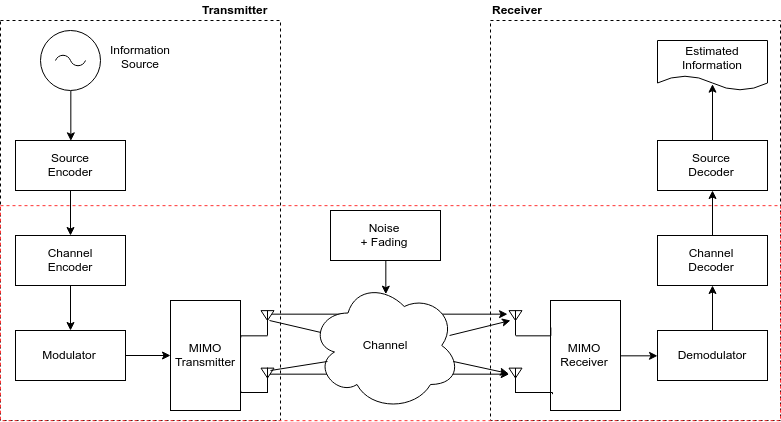
\includegraphics[width=\textwidth]{resources/systemDiagram.png}
	\caption{System block diagram of a typical communication system with MIMO architecture}
	\label{fig:sys}
\end{figure}{}
\\
From figure \ref{fig:sys}, it can be seen that the receiver mirrors the transmitter in most of the sub-components. 

\subsection{The Transmitter}
\label{sub:trans}

On the transmitter side, the source encoder takes in a raw message signal and converts it into a sequence of bits. This is done to compress the raw message data and to remove redundancy. The end result of source encoding is digital information bits with lesser bandwidth and just enough information to reconstruct the original message \cite{B10}. After source encoding, the information bits are sent to the channel encoder. The channel encoder uses FEC codes to add redundancy to the information bits. This is done to facilitate error detection and correction on the receiver side after channel transmission. The next step is modulation, the modulator takes in the coded bits from the channel encoder and maps them to a signal to be transmitted over the channel. This is done to conserve power and bandwidth. The MIMO transmitter takes in the symbols and transmits them over the channel using its multiple antennas. The MIMO transmitter uses multiple antennas to boost bandwidth and to improve signal range as mentioned earlier.

\subsection{The Channel}
The steps mentioned in section \ref{sub:trans} are taken so as to  prepare the original message to prevail in the channel and so that it is sent as efficiently as possible. The channel can be any medium, wireless or physical, into which the transmitted signal propagates. The channel distorts and adds noise to the transmitted signal, and in some instances interference occurs \cite{B10}. 

\subsection{The Receiver}
The mirrored side of of the transmitter, which is the receiver, performs the opposite of all the steps mentioned in section \ref{sub:trans} respectively. This done in order to recover the original sent message to the highest accuracy possible. 
\\
\\
This paper only focuses on the part of the communication system highlighted in red on figure \ref{fig:sys}.

\section{Channel Encoding}
\label{sec:encoding}
As mentioned earlier, transmitting data over a noisy channel often leads to the information being corrupted. To minimise the occurrence of errors during transmission the information has to somehow be protected. This protection is achieved through either the use of FEC codes or Automatic Repeat Requests (ARQ). ARQ requires retransmission of bits if they are in error. This leads to delays in communication, wasteful retransmissions that require additional power and bandwidth and also interference with other users \cite{B11}. All these make ARQ not suitable for real-time applications especially in interactive media applications \cite{51}. FEC on the other hand uses error correcting codes to correct errors that occur during transmission. It does this by adding redundant bits on the information bits, this helps to detect and correct errors as mentioned earlier. For this design FEC is chosen due to the fact that it offers improved BER, higher throughput and minimal delays compared to its counterpart \cite{51,52}.
\\
\\
FEC codes are split up into two categories: Convolutional Codes and Linear Block Codes. Error correcting capability and/or performance of an FEC coding scheme is measured by its code rate $r$. The code rate represented by equation \ref{eq:1} below.

\begin{equation}
r = \frac{k}{n}
\label{eq:1}
\end{equation}{}
\\
The code rate presents the proportion of the data stream that is useful to the one that has redundancy, represented by $k$ and $n$ respectively in equation \ref{eq:1}.

\subsection{Convolutional Codes}
\label{sub:conv}
Convolutional Codes are mostly used in applications that require real time error correction. They are generated by combining the input data stream bits in a series manner. The input bits are stored in a fixed length shift register and are combined with the use of modulo-2 adders \cite{53}. The output of the convolutional encoder at any point is a combination of the previous bits in the shift register.
\\
\\
One type of a Convolutional Codes are Turbo codes. Turbo codes are known to perform extremely well compared to any other FEC code. They achieve within a fraction of a dB of the Shannon Capacity in certain channels \cite{B11}. The major disadvantage of Convolutional Codes is their complexity. The complexity curve steepens even further when trying to decode them \cite{B11}. The simplest decoder which is the Viterbi also increase in complexity and it gets much difficult to implement for large codewords
\cite{54}.

\subsection{Linear Block Codes}
In Linear Block Codes, the resultant codeword is formed as a linear combination of two codewords. The two codewords are the original message bits having size $k$ and the parity bits of size $n-k$, where $n$ is the size of the resulting codeword.
\\
\\
There exist three main types of of Linear Block Codes used in coding theory: Bose Chaudhuri Hochquenghem (BCH), Reed Solomon (RS) and Low Density Parity Check (LDPC) codes. LDPC codes are regarded to be in the same league as Turbo codes with regards to performance. However, like Turbo codes they have major draw backs. LDPC codes require large sums of computation power, have low flexibility and have high encoding complexities \cite{59,56}.  RS codes, derived from BCH codes, are well known for their suitability when it comes to correcting burst errors. Compared with BCH, they were found to perform poorly in RFCs \cite{10,57}. Due to arguments raised in section \ref{sub:conv} and in this section BCH codes are chosen as the suitable candidate for this design.
\\
\\
BCH codes form a class of cyclic codes constructed using the principles of the Galois Finite Fields. Unlike RS codes, they are able to correct multiple random errors and unlike LDPC and Turbo codes, they are relatively easier to implement and decoding is also simple \cite{20,57}. Other great advantages of this coding scheme is its flexibility of choosing the number of errors correctable by the code and its great error correcting capabilities \cite{57,58,22}.

\subsubsection{BCH Encoder and Decoder}
BCH$(n,k)$ codes are a generalisation of Hamming Code. Unlike Hamming code, BCH$(n,k)$ posses the ability to correct multiple errors. They are described mathematically as follows:

\begin{center}
\begin{minipage}[h!]{0.85\textwidth}
  	
  	
  	{\it For any positive integers $m\ge3$ and $ t < 2^{m-1} $ there exists a BCH(n,k) code with the following characteristics:}
  	
  	\begin{equation}
  	\label{eq:block}
  	 \mbox{Block length: \hspace{1cm}} n = 2^{m-1}  	
  	\end{equation}
  	\begin{equation}
  	\label{eq:parity}
  	\mbox{Parity check bits: \hspace{1cm}} n -k \le mt 	
  	\end{equation}
  		\begin{equation}
  	\label{eq:dmin}
  	\mbox{Minimun distance: \hspace{1cm}} d_{min} \ge 2t + 1	
  	\end{equation}

\end{minipage}
\end{center}

A BCH$(n,k)$ code described by equations \ref{eq:block}$-$\ref{eq:dmin} is described as a $t$-error correcting BCH.
\\
\\
To encode, BCH codes uses a generator polynomial $g(x)$ defined in the Galois Field GF($2^m$). The polynomial is the lowest degree polynomial over GF(2) which has $\alpha, \alpha^2,...,\alpha^{2t}$ as its roots. If $\Phi(x)_i$ is a minimal polynomial of $\alpha_i$, then $g(x)$ is given by equation \ref{eq:gx} below,

\begin{equation}
\label{eq:gx}
	g(x) = LCM(\Phi(x)_1,\Phi(x)_3,...,\Phi(x)_{2t-1})
\end{equation}
\\
A more detailed mathematical derivation of how equation \ref{eq:gx} is obtained can be found here \cite{B13}. The codeword $c(x)$ is formed by first dividing the message polynomial $m(x)$ and obtaining the remainder $r(x)$. The remainder $r(x)$ is then added to original message polynomial $m(x)$ to make the output codeword $c(x)$ as described by equation \ref{eq:rx}--\ref{eq:cx}.

\begin{equation}
\label{eq:rx}
r(x) = mod\{m(x),g(x)\}
\end{equation}
\begin{equation}
\label{eq:cx}
c(x) = m(x) + r(x)
\end{equation}
\\
To decode BCH codewords, there a four main steps that are followed:
\begin{enumerate}[i]
	\item Syndrome computation
	\item Determine coefficients of the error locator polynomial. 
	\item Find the roots of the error locator polynomial.
	\item Correct the error
\end{enumerate}
The steps above are described mathematically and in more detail by \cite{59,21,EXS}. In this design BCH$(127,85)$ code with parameters described in table \ref{t:bch} is used.

\begin{table}[h!]
	\caption{BCH(127,85) paramaters}
	\label{t:bch}
	\begin{tabular}{|l|l|l|l|l|l|l|}
		\hline
		\textbf{Parameter} & m & n & k & t & r & \multicolumn{1}{c|}{$g(x)$} \\ \hline
		\textbf{Value} & 6 & 127 & 85 & 6 & 0.67 & \begin{tabular}[c]{@{}l@{}}$1 + x + x^{3} + x^{4} + x^{5} + x^{7} + x^{10} + x^{13} + x^{15} + x^{16} + x^{19} + x^{20} +$\\ $x^{21} + x^{22} + x^{23} + x^{26} + x^{29} + x^{33} + x^{34} + x^{35} + x^{39} + x^{40} + x^{42}$\end{tabular} \\ \hline
	\end{tabular}
\end{table}{}

From the table it can be seen that BCH$(127,85)$ has a code rate of 0.67 as per equation \ref{eq:1} and it can correct up-to 6 errors. The encoder and decoder are both implemented in MATLAB.

\newpage

\section{Digital Modulation}
\label{sec:modem}
 
%% References
\bibliographystyle{IEEEtrans}
\bibliography{references}




\end{document}          
